\documentclass[12pt]{article}

\usepackage{fontspec}
\usepackage{polyglossia}
\usepackage{geometry}
\usepackage{graphicx}

\usepackage{amsmath,
            amsthm,
            amssymb
}

\usepackage{unicode-math,
            tensor
}

\usepackage{wrapfig, 
            hyperref,
            multicol,
            multirow,
            tabularx,
            booktabs,
            makecell
}

\usepackage{}

\geometry{a4paper,
          total={170mm,255mm},
          left=10mm,
          top=15mm,
}

\setdefaultlanguage{russian}
\setotherlanguage{english}
\setkeys{russian}{babelshorthands=true}

\defaultfontfeatures{Ligatures=TeX}
\setmainfont{STIX Two Text}
\setmathfont{STIX Two Math}
\DeclareSymbolFont{letters}{\encodingdefault}{\rmdefault}{m}{it}

\newfontfamily{\cyrillicfont}{STIX Two Text} 
\newfontfamily{\cyrillicfontrm}{STIX Two Text}
\newfontfamily{\cyrillicfonttt}{Courier New}
\newfontfamily{\cyrillicfontsf}{STIX Two Text}

\renewcommand{\thefigure}{\thesection.\arabic{figure}}
\renewcommand{\thetable}{\thesection.\arabic{table}}
\numberwithin{equation}{section}

\renewcommand{\qedsymbol}{$\blacksquare$}
\theoremstyle{definition}
\newtheorem{definition}{Опр.}[section]
\theoremstyle{remark}
\newtheorem{statement}{Утв.}[section]
\theoremstyle{plain}
\newtheorem{theorem}{Теор.}[section]

\addto\captionsrussian{
  \renewcommand{\figurename}{Рис.}
  \renewcommand{\tablename}{Табл.}
  \renewcommand{\proofname}{Док-во}
}

\graphicspath{{./img/}}
\everymath{\displaystyle}

\newcommand{\RNumb}[1]{\uppercase\expandafter{\romannumeral#1\relax}}
\newcommand{\llabel}[1]{\label{\thesubsection:#1}}
\newcommand{\lref}[1]{\ref{\thesubsection:#1}}
\begin{document}
\paragraph{Э-16}
Движущийся со скоростью $\vec v$ электрон, попадает в однородные и взаимно перпендикулярные электрическое $\vec E$ и магнитное $\vec B$ поля. Скорость электрона перпендикулярна обоим полям. Найдите траекторию движения электрона.\\

Мы не черти, мы решаем нерелятивистский случай. А значит $\nu \ll 1$.\\
$\vec H || \vec (OZ)$ и $\vec E || \vec (OY)$.\\
Тогда уравнения движения будут иметь вид:
$$
m\dot{\vec\nu} = e\vec E+e\vec\nu\times\vec H,
$$
Или, в нашем случае:
\begin{gather*}
\begin{cases}
m\ddot x= e\dot y H \\
m\ddot y = eE_y-e\dot x H=eE-e\dot x H \\
m\ddot z = eE_z=0
\end{cases},
\end{gather*}

\begin{wrapfigure}[34]{r}{0.3\linewidth}
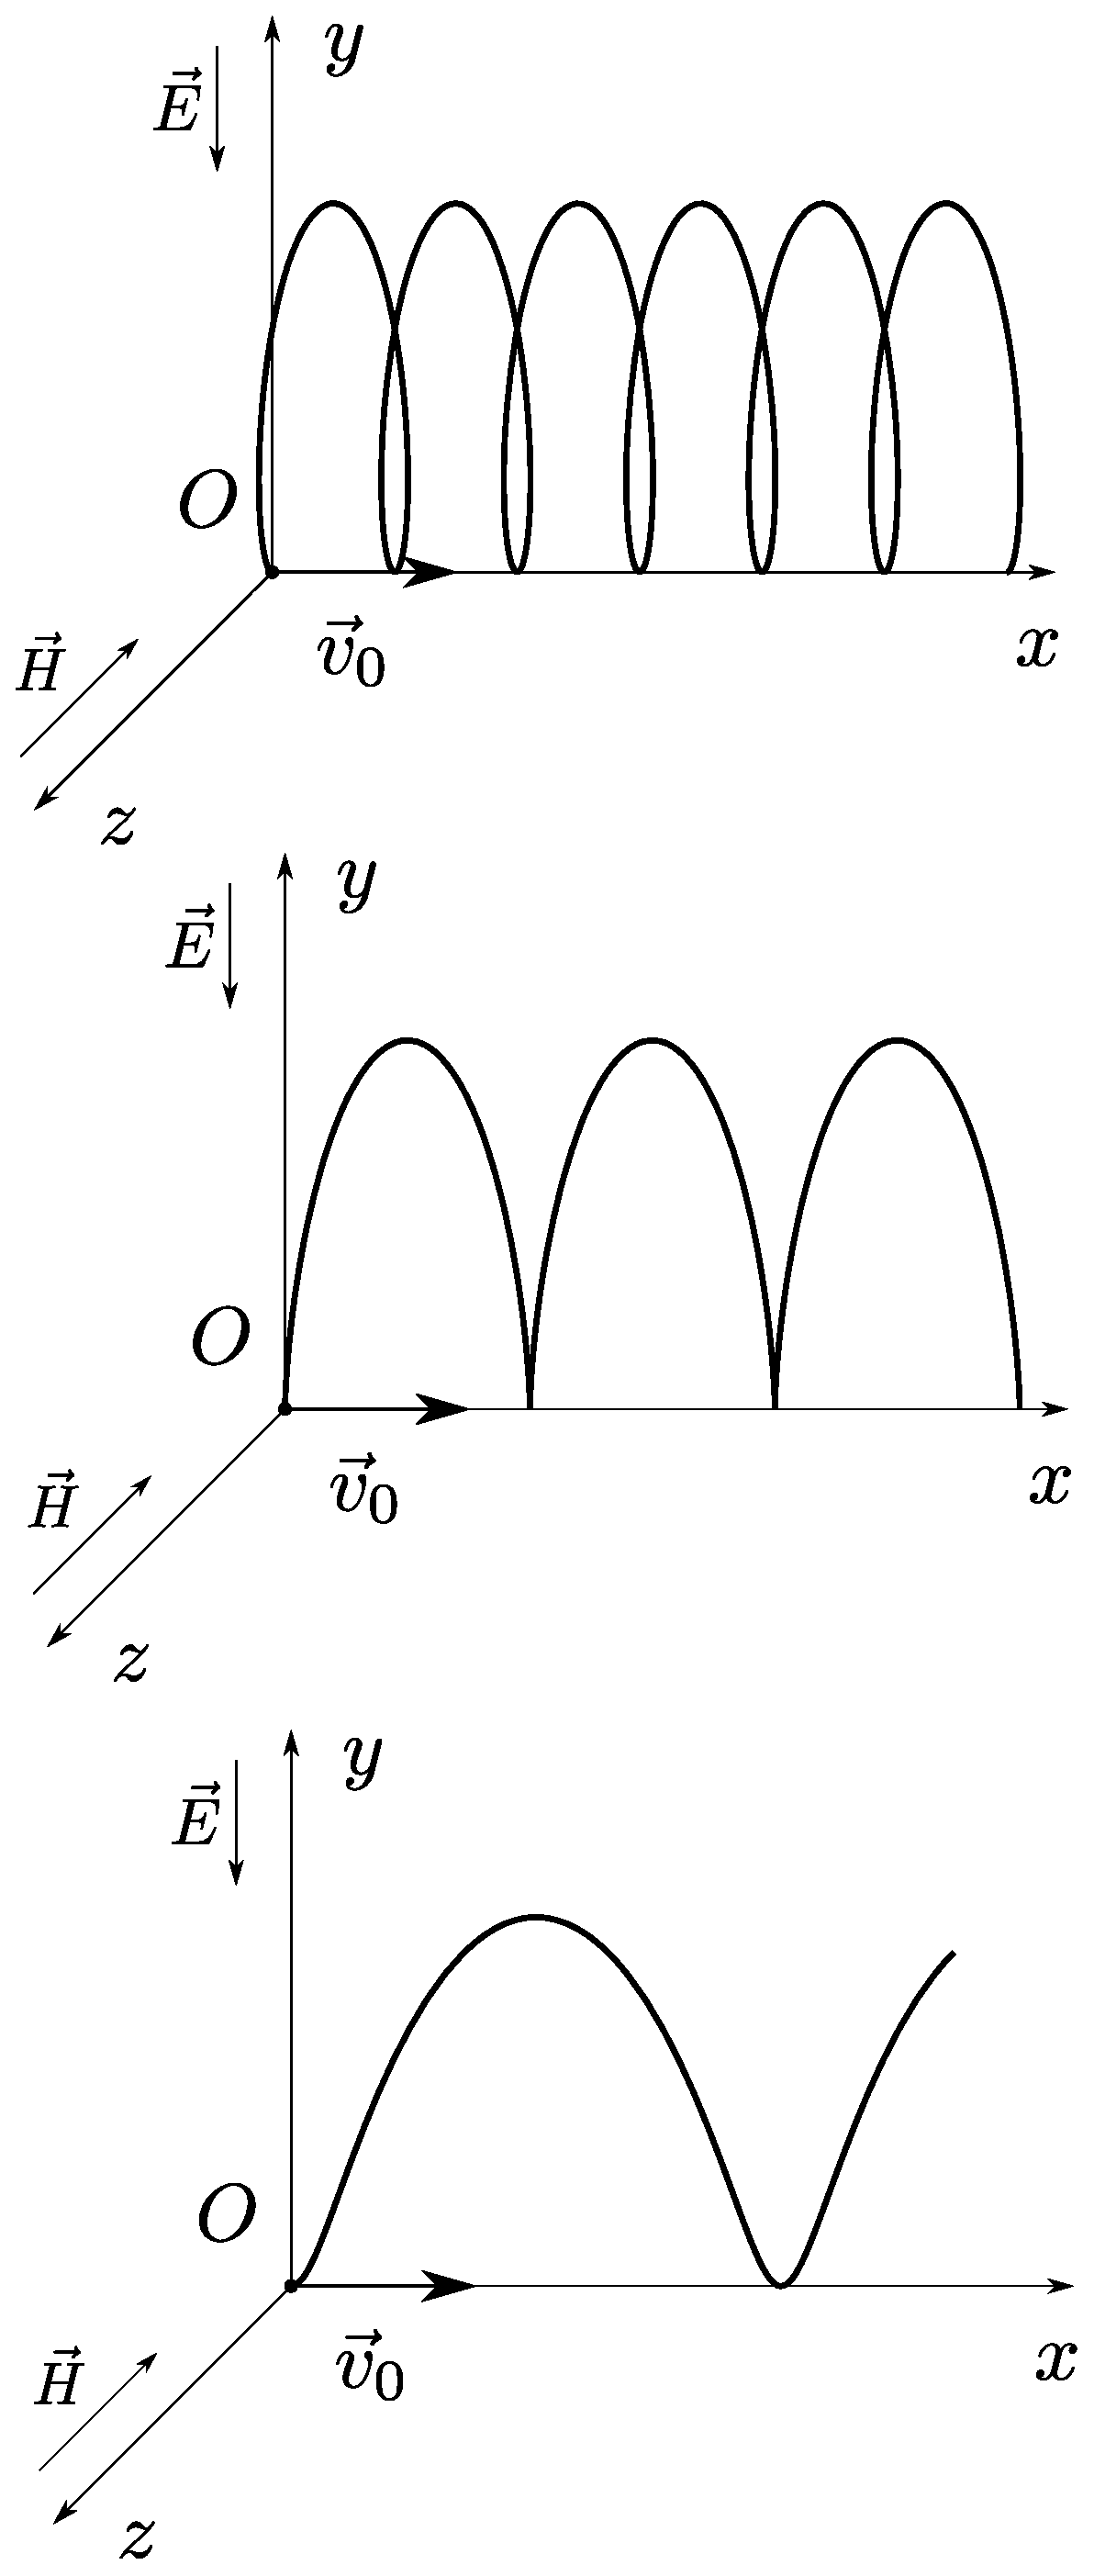
\includegraphics[width=1\linewidth]{img/e-16.eps}
\caption{Качественно различные траектории частицы.}
\end{wrapfigure}

У множим второе уравнение (для $\ddot y$) на $i$ и сложим с первым, положив $\dot z = \dot x + i \dot y$:
$$
\frac{d}{dt}\dot z+i\omega\dot z = i\frac{e}{m}E
$$
Где $\omega = \frac{eH}{m}$. Решение этого дифференциального уравнения примет вид:
$$
\dot x + i\dot y=\alpha e ^{-i\omega t}+\frac{E}{H}
$$

В общем случае $\alpha$ - комплексное число, однако правильно выбрав начало отсчета времени мы можем сделать так, что умножение на $e^{-i\omega t}$ избавит нас от хлопот, и, как следствие, сделает $\alpha$ действительным.\\

Отделяя комплексные переменные от действительных получим пару уравнений:
\begin{flalign*}
\begin{split}
\dot x &= \alpha \cos(\omega t)+ \frac{E}{H} \\
\dot y &= -\alpha \sin(\omega t)
\end{split},
\end{flalign*}

Очевидно , что
\begin{flalign*}
\begin{split}
x &= \frac{\alpha}{\omega} \sin(\omega ct)+ \frac{Ect}{H}\\
y &= \frac{\alpha}{\omega} \cos(\omega ct-1)
\end{split}
\end{flalign*}

Пределы интегрирования выставлялись так, что $x(0)=y(0)=0$.\\
Собственно, в зависимости от соотношения параметров параметрических уравнений возможно три качественно различных случая, которые и изображены на рисунках.

Ах да, нам дан вектор $\vec B=\vec H..... $
\end{document}